\documentclass[runningheads]{llncs}

\usepackage[T1]{fontenc}
\usepackage{graphicx}
\usepackage{amsmath}
\usepackage{amssymb}
\usepackage{booktabs}
\usepackage{xcolor}
\usepackage{listings}
\usepackage{tikz}
\usepackage{microtype}
\usepackage{url}
\usetikzlibrary{shapes.geometric, arrows.meta, positioning, fit, backgrounds}

% ── Listings: Spectre language ────────────────────────────────────────────────
\definecolor{spectreblue}{RGB}{0,70,150}
\definecolor{spectregreen}{RGB}{0,120,60}
\definecolor{spectregray}{RGB}{100,100,100}
\definecolor{spectrebg}{RGB}{248,248,252}

\lstdefinelanguage{Spectre}{
  morekeywords={var, const, param, init, action, require, invariant, temporal,
                always, eventually, next, until, WF, SF, enum,
                description, import, as, oneOf, forAll, exists},
  morekeywords=[2]{true, false},
  sensitive=true,
  morecomment=[l]{//},
  morestring=[b]"
}

\lstset{
  language=Spectre,
  basicstyle=\ttfamily\small,
  keywordstyle=\color{spectreblue}\bfseries,
  keywordstyle=[2]\color{spectregreen}\bfseries,
  commentstyle=\color{spectregray}\itshape,
  stringstyle=\color{spectregreen},
  backgroundcolor=\color{spectrebg},
  frame=single,
  framerule=0.4pt,
  xleftmargin=6pt,
  xrightmargin=6pt,
  numbers=left,
  numberstyle=\tiny\color{spectregray},
  numbersep=5pt,
  breaklines=true,
  captionpos=b,
  showstringspaces=false,
  tabsize=2
}

\lstdefinelanguage{Rust}{
  morekeywords={pub, fn, struct, enum, impl, let, mut, self, Self,
                use, mod, return, if, else, match, for, while, loop,
                true, false, assert, assert_eq, i64, u64, i32, bool, String},
  sensitive=true,
  morecomment=[l]{//},
  morestring=[b]"
}

% ── TikZ styles ───────────────────────────────────────────────────────────────
\tikzset{
  box/.style={rectangle, rounded corners=3pt, draw=black!60, fill=white,
              minimum height=1.8em, minimum width=5em, align=center,
              font=\small},
  bigbox/.style={rectangle, rounded corners=4pt, draw=black!40, fill=gray!8,
                 minimum height=1.8em, align=center, font=\small},
  arr/.style={-{Stealth[length=5pt]}, thick},
  dasharr/.style={-{Stealth[length=5pt]}, thick, dashed, gray},
}

% ─────────────────────────────────────────────────────────────────────────────
\begin{document}

\title{Spectre: Closed-Loop Refinement, Repair, and Conformance for Rust}
\titlerunning{Spectre: Closed-Loop Refinement, Repair, and Conformance}

\author{Anonymous Author(s)}
\authorrunning{Anonymous}

\institute{Institution omitted for blind review}

\maketitle

% ── Abstract ──────────────────────────────────────────────────────────────────
\begin{abstract}
We present \textsc{Spectre}, a formal-methods toolchain that derives a
refinement mapping from Rust source and maintains it throughout model checking,
counterexample-guided repair, conformance testing, and runtime monitoring.
AST-based mining from a Rust \texttt{struct}/\texttt{impl} pair produces both
a Spectre model and a Rust\,--\,model field/action correspondence
(\emph{refinement map}) with no manual model-skeleton or correspondence effort.
A CEGIS repair engine synthesises weakest-precondition guards for simultaneous
assignments, Boolean/enum conditions, and aggregates constraints across multiple
counterexamples into conjunctive guards.
The refinement map drives automatic generation of ITF conformance tests,
Rust \texttt{\#[test]} regression tests, and coverage-guided MBT traces
(action, transition-pair, boundary, rare-action, and property-directed modes).
\texttt{spectre sync} detects drift by comparing fields, actions, guards, and
normalised assignment expressions, detecting \textbf{30/35 injected mutations}
(85.7\%); when one action changes, \texttt{verify -{}-incremental} incrementally
updates and re-verifies the reachable-state graph---\textbf{3.0--3.6$\times$ faster} than cold BFS on the
22{,}432-state Raft model (8.7\,s cold BFS on our benchmark platform, 2.4--2.9\,s
incremental); cache restore for an unchanged spec takes 0.26\,s
(\textbf{33$\times$ faster}).
Direct simulation (\texttt{spectre simulate}) samples execution paths
without constructing the full graph, covering 5- and 7-node Raft
configurations beyond BFS scale.
Evaluation on 10 Rust components confirms 36/36 guards correctly mined,
10/10 positive MBT traces replayed, 2/2 injected implementation faults
detected, and WP repair in under 6\,s across arithmetic, Boolean, enum,
and simultaneous assignment forms.

\keywords{Formal specification \and Refinement \and Program synthesis \and
  CEGIS \and Model-based testing \and Runtime monitoring \and Rust}
\end{abstract}

% ── 1. Introduction ───────────────────────────────────────────────────────────
\section{Introduction}\label{sec:intro}

Formal specification has demonstrated its value at scale: Amazon Web Services
reports using TLA+ and model checking to uncover subtle design errors in
critical distributed systems before implementation and deployment~\cite{newcombe2015amazon}.
Yet adoption remains narrow.
The principal barrier is not expressiveness but ergonomics: TLA+ uses
mathematical notation unfamiliar to systems programmers~\cite{wing1990specifier},
and even Quint---which maps TLA+ concepts to a TypeScript-like syntax---remains
specification-first: the implementation--model bridge is supplied separately by
the user, and neither Quint nor TLA+ provides deterministic weakest-precondition
repair or a Rust-AST-derived correspondence.

Three practical limitations restrict wider adoption.
First, \emph{specification authoring cost}: expressing a full system model in
an unfamiliar notation, starting from scratch.
Second, \emph{manual guard discovery}: when the model checker reports a
violation, identifying and inserting the missing precondition by hand.
Third, \emph{specification drift}: once verified, specification and
implementation can evolve independently with limited tooling to detect or
recover from divergence.

We present \textsc{Spectre}, an open-source formal-methods toolchain that
addresses all three stages.
Unlike specification-first workflows (Quint, TLA+) where the
model--implementation bridge is manually supplied, Spectre derives this
correspondence from Rust source and reuses it throughout verification, repair,
testing, synchronisation, and runtime monitoring.
Spectre's central contribution is a \emph{source-derived refinement map} that
connects Rust implementation states and transitions to the formal model, and is
maintained across the full development lifecycle.

\smallskip\noindent\textbf{C1: Source-derived refinement and incremental synchronisation.}
\texttt{mine -o} produces a Spectre model plus a Rust--model
field/action correspondence from Rust ASTs.
\texttt{sync} classifies code changes as \emph{structurally unchanged},
\emph{spec-update-required}, or \emph{possibly-unsafe}, comparing fields,
actions, guard counts, guard expressions, and normalised assignment expressions;
semantic changes not visible in the current normalised representation remain
a limitation.
\texttt{drift} detects bidirectional staleness.

\smallskip\noindent\textbf{C2: Counterexample-guided repair with validation.}
WP synthesis over simultaneous assignments, Boolean/enum guards, and
multiple counterexamples; trace-preserving repair validation that flags
over-restrictive guards before application.

\smallskip\noindent\textbf{C3: Generated conformance and regression infrastructure.}
\texttt{spectre check-refinement} classifies implementation transitions as
legal, stuttering, or violating; coverage-guided ITF trace generation
(action, transition-pair, boundary, rare-action, and property-directed modes);
automatic \texttt{\#[test]} generation from counterexamples.

\smallskip\noindent\textbf{C4: Scalable exploration.}
\texttt{spectre simulate} for direct path sampling without full graph construction;
\texttt{param N: int} for parameterised models enabling scale-sweep
verification (e.g., 3-/5-/7-node Raft).

Sections~\ref{sec:arch}--\ref{sec:conformance} present the architecture,
repair, sync, and testing components; \S\ref{sec:eval} evaluates;
\S\ref{sec:related}--\ref{sec:conclusion} discuss related work and conclude.

% ── 2. Source-Derived Refinement Architecture ─────────────────────────────────
\section{Source-Derived Refinement Architecture}\label{sec:arch}

\paragraph{Kripke Structures and Bounded Checking.}
A \emph{Kripke structure} $M = (S, S_0, R, L)$ has states $S$, initial states
$S_0 \subseteq S$, a transition relation $R \subseteq S \times S$, and a
labelling function $L$~\cite{clarke1986automatic}.
Spectre constructs $M_\Sigma$ by BFS from $S_0$, evaluating all enabled
actions and checking invariants on each transition.
\texttt{always(P)} requires $P$ in every explored state.
\texttt{eventually(P)} reports a \emph{bounded witness}:
$\exists\pi.\,\exists i \le k{:}\;M,\pi_i \models P$, i.e., bounded
existential reachability, not the universal LTL property $M \models \lozenge P$~\cite{pnueli1977temporal}.
Full automata-based LTL over infinite paths and WF/SF checking are future work.

\paragraph{The Refinement Map.}
Let $\Sigma_M$ be the Spectre model state space and $\Sigma_I$ the Rust
implementation state space.
A \emph{refinement map} $\mathcal{R} \subseteq \Sigma_I \times \Sigma_M$
relates implementation states to model states via a field projection $\pi$:
for $(s_I, s_M) \in \mathcal{R}$, each spec variable maps to the
corresponding Rust field value.
An implementation transition $(s_I \to t_I)$ \emph{conforms} to $\mathcal{R}$
if either: (i)~there exists a model action $A$ such that $(s_I,s_M)\in\mathcal{R}$,
$(t_I,t_M)\in\mathcal{R}$, all \texttt{require} guards of $A$ hold in $s_M$,
and $s_M \xrightarrow{A} t_M$ is a legal Spectre transition; or
(ii)~the step is a \emph{stuttering step}: $\pi(s_I) = \pi(t_I)$ (all
spec-relevant fields unchanged).

\begin{proposition}[Refinement Conformance]\label{prop:refine}
If \texttt{check-refinement} returns \emph{Legal} for a trace transition
and the field/action map is faithful, then the corresponding Spectre action
is enabled in $s_M$, all \texttt{require} guards hold in $s_M$, and
$\pi(t_I) = t_M$ (projected post-states agree).
\end{proposition}

\noindent\textit{Scope.}  This is trace-level conformance --- it verifies
every supplied transition, not all possible implementation executions.

\paragraph{Source Derivation.}
\texttt{spectre mine -o spec.spec src.rs} produces two artefacts: a
\texttt{.spec} file containing the formal model, and a \emph{refinement map
file} (\texttt{.driver.json}) recording the field/method correspondence.
The AST miner~\cite{syncratedoc} maps struct fields to \texttt{var}
declarations, constructor literals to \texttt{init} values,
\texttt{assert!} calls and early-return guards to \texttt{require} guards,
and field assignments to primed transitions.  This derivation is
the key automation enabling automatic refinement checking: no user-supplied
state-extraction or transition-reproduction code is required.
The mined model faithfully reflects the Rust implementation; correctness
properties (\texttt{invariant} and \texttt{temporal} declarations) must be
supplied independently to avoid a circular oracle where implementation bugs
are reproduced verbatim in the model.

\paragraph{Spectre Language.}
A Spectre specification declares typed state variables with \texttt{var},
an initial state with \texttt{init}, and guarded actions with \texttt{action}.
An action lists \texttt{require} guards (preconditions) followed by
primed-variable assignments (\texttt{x'~=~expr}).  Disabled actions are
silently skipped; unmentioned variables retain their value (frame condition).
Parameterised models declare \texttt{param N: int} and bind values at
verification time via \texttt{-{}-param N=5}, enabling scale-sweep experiments.
Actions with \texttt{int} parameters are instantiated over $[-5,5]$ by default
(\texttt{-{}-param-bound} configurable); \texttt{-{}-max-states} and
\texttt{-{}-max-depth} cap exploration.

Table~\ref{tab:comparison} compares Spectre with TLA+ and Quint across the
features most relevant to the closed-loop lifecycle.
Figure~\ref{fig:arch} shows the full pipeline.

\begin{table}[t]
\caption{Feature comparison of formal specification tools (open-source/core
  toolchains; commercial services excluded).}\label{tab:comparison}
\centering
\begin{tabular}{lccc}
\toprule
Feature                              & TLA+ & Quint & \textsc{Spectre} \\
\midrule
Infinite-trace temporal checking     & \checkmark & \checkmark & --$^\diamond$ \\
Bounded temporal checking            & \checkmark & \checkmark & \checkmark \\
Type inference                       & --         & \checkmark & \checkmark \\
WP guard synthesis                   & --         & --         & \checkmark \\
Source-derived Rust\,--\,model map  & --         & partial$^\dagger$ & \checkmark \\
Incremental sync / drift detection   & --         & --         & \checkmark \\
Runtime monitor generation           & --         & --         & \checkmark \\
Coverage-guided MBT traces           & --         & $\circ$$^\star$ & \checkmark \\
Parameterised models                 & \checkmark & \checkmark & \checkmark \\
Self-loop / livelock detection       & --         & --         & \checkmark \\
\bottomrule
\multicolumn{4}{l}{\small $^\dagger$Quint Connect requires user-supplied state extraction and step mapping.} \\
\multicolumn{4}{l}{\small $^\diamond$Bounded-prefix checking; full LTL, WF, and SF are future work.} \\
\multicolumn{4}{l}{\small $^\star$Quint: random sim.\ + \texttt{-{}-n-traces}; action/boundary/rare-action modes absent.} \\
\end{tabular}
\end{table}

\begin{figure}[t]
\centering
\resizebox{\columnwidth}{!}{%
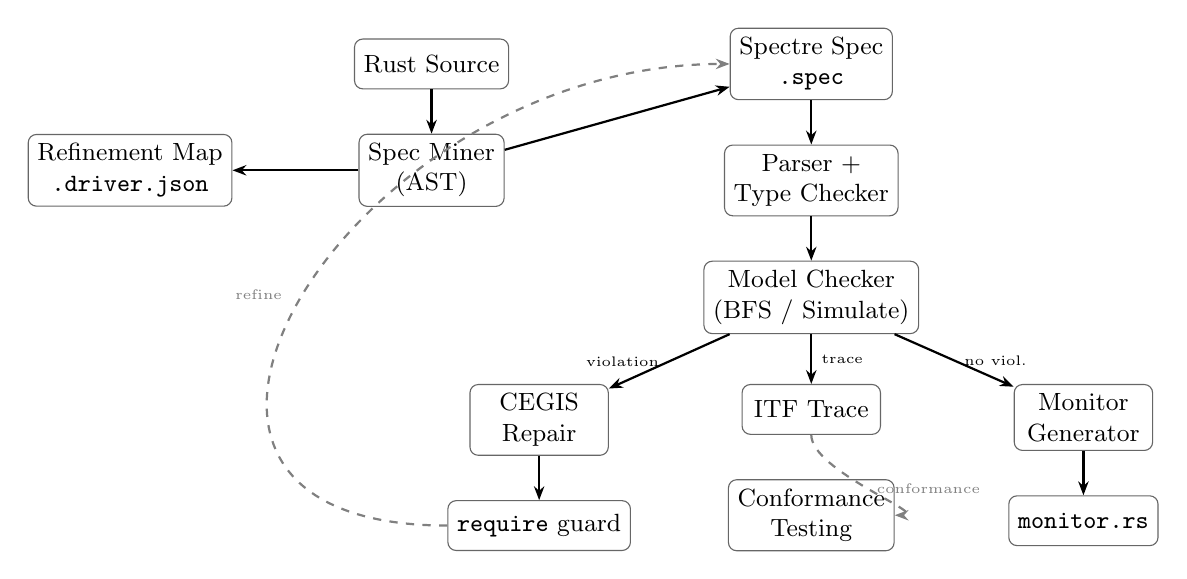
\begin{tikzpicture}[node distance=1.6em and 1.8em]
  % Row 1: inputs
  \node[box] (rust)   {Rust Source};
  \node[box, right=2.8cm of rust] (spec) {Spectre Spec\\\texttt{.spec}};

  % Row 2: processing
  \node[box, below=of rust] (miner)  {Spec Miner\\(AST)};
  \node[box, below=of spec] (parser) {Parser +\\Type Checker};

  % Row 3: core
  \node[box, below=of parser] (mc) {Model Checker\\(BFS / Simulate)};

  % Row 4: outputs
  \node[box, below left=1.8em and 1.2cm of mc] (cegis)   {CEGIS\\Repair};
  \node[box, below=1.8em of mc]               (itf)     {ITF Trace};
  \node[box, below right=1.8em and 1.2cm of mc](monitor){Monitor\\Generator};

  % Row 5: final outputs
  \node[box, below=of cegis]   (req)   {\texttt{require} guard};
  \node[box, below=of itf]     (driver){Conformance\\Testing};
  \node[box, below=of monitor] (mon)   {\texttt{monitor.rs}};

  % Refinement map produced by miner
  \node[box, left=1.6cm of miner] (driverout) {Refinement Map\\\texttt{.driver.json}};

  % Arrows
  \draw[arr] (rust)   -- (miner);
  \draw[arr] (miner)  -- (spec);
  \draw[arr] (miner)  -- (driverout);
  \draw[arr] (spec)   -- (parser);
  \draw[arr] (parser) -- (mc);
  \draw[arr] (mc)     -- node[left,  font=\tiny]{violation} (cegis);
  \draw[arr] (mc)     -- node[right, font=\tiny]{trace}     (itf);
  \draw[arr] (mc)     -- node[right, font=\tiny]{no viol.}  (monitor);
  \draw[arr] (cegis)  -- (req);
  \draw[dasharr] (itf) to[out=-90,in=0,looseness=0.8]
    node[right, font=\tiny]{conformance} (driver);
  \draw[arr] (monitor)-- (mon);

  % Feedback arrow
  \draw[dasharr] (req) to[out=180,in=180,looseness=1.8]
    node[left, font=\tiny, xshift=-4pt]{refine} (spec);
\end{tikzpicture}}%
\caption{Spectre architecture.  \texttt{spectre mine} produces both the
Spectre model and the Refinement Map (\texttt{.driver.json}) from the Rust
AST.  The model checker feeds violations to CEGIS repair and traces to
conformance testing; \texttt{sync} and \texttt{drift} use the Refinement Map
for incremental re-verification.}\label{fig:arch}
\end{figure}

% ── 3. Counterexample-Guided Repair with Trace-Preservation Validation ────────
\section{Counterexample-Guided Repair with Trace-Preservation Validation}\label{sec:cegis}

\paragraph{Algorithm.}
Spectre implements a counterexample-guided refinement loop~\cite{solar2008program,alur2013syntax}
for guard synthesis.  Given violated invariant $\mathit{inv}$ and counterexample
ending with action $A$ in pre-state $\sigma_{k-1}$, Spectre computes
$g = \mathrm{wp}(A, \mathit{inv})$~\cite{dijkstra1976discipline}
by syntactic substitution.  The candidate guard is added as a \texttt{require}
clause and the model is re-explored; the loop iterates until no violation is
found within the configured state budget or a fixed-point is reached.
The iterative loop is not guaranteed to converge in general; in practice each
iteration eliminates at least the current counterexample.

\paragraph{Extended Synthesis.}
All assignment forms are handled uniformly by substitution.
For an action with simultaneous assignments $\{x_1' = e_1, \ldots, x_n' = e_n\}$
and invariant $I$:
\[
\mathrm{wp}(\{x_i' = e_i\},\; I)
  \;=\; I[x_1 \leftarrow e_1,\;\ldots,\; x_n \leftarrow e_n]
\]
Boolean ($b' = \mathit{true/false}$) and enum ($e' = V$) assignments are
syntactic instances of $x' = e$: after substitution the expression may reduce
to a constant, in which case the guard is omitted ($\mathit{true}$) or the
action is statically disabled ($\mathit{false}$).
\texttt{AccumulateGuards} aggregates distinct WP conditions across counterexamples
for the same (invariant, action) pair.

\paragraph{Formal Guarantees.}

\begin{proposition}[Substitution Soundness]\label{prop:wp}
Let $I$ be an invariant and $A$ an action with simultaneous assignments
$\{x_1' = e_1, \ldots, x_n' = e_n\}$.  Let
$g = I[x_1 \leftarrow e_1, \ldots, x_n \leftarrow e_n]$
be the result of simultaneous syntactic substitution.
For any pre-state $\sigma$: if $\sigma \models g$ then $A(\sigma) \models I$.
This holds for all supported assignment forms; arithmetic, Boolean, and enum
assignments are syntactic instances.
\end{proposition}

\begin{corollary}[Trace-Preserving Repair Validation]\label{cor:repair}
Let $g$ be a guard synthesised by WP substitution for assignments
$\{x_i' = e_i\}$ against invariant $I$.
(i)~\textbf{Soundness.}  Adding $g$ as a \texttt{require} clause prevents the
violating transition.
(ii)~\textbf{Trace preservation.}  The \texttt{-{}-check-repair-minimal}
checker validates that $g$ does not block any transition present in supplied
positive traces; a guard that would block a known-good step is flagged as
over-restrictive.  This is positive-trace preservation, not global minimality.
\end{corollary}

\paragraph{Causal Diagnosis.}
For each counterexample, Spectre computes: the first divergence point (earliest
step where the WP condition was unsatisfied), the responsible variable set
(variables referenced in the violated invariant clause that changed along
the path), and the candidate fix in Spectre syntax.  This structured output
replaces verbose trace dumps and is reported immediately after each violation.

% ── 4. Incremental Synchronisation and Verification ──────────────────────────
\section{Incremental Synchronisation and Verification}\label{sec:sync}

Code and specifications drift.
Spectre provides three mechanisms to detect and recover from drift without
full re-exploration.

\paragraph{Bidirectional Drift Detection (\texttt{spectre drift}).}
The refinement map file records field and method names at mine time.
\texttt{spectre drift} compares the current Rust source against this record
and reports: (a)~Rust fields with no matching spec variable; (b)~spec
variables with no Rust implementation correspondence; (c)~invariants
that may need monitor regeneration.  The check is $O(|F|+|A|)$ in the number
of fields and actions and completes in milliseconds.

\paragraph{Incremental Synchronisation (\texttt{spectre sync}).}
\texttt{spectre sync} re-mines the Rust source and classifies each
change against the existing spec:
\begin{itemize}
  \item \emph{Structurally unchanged}: same variables, same actions, same guard
    counts, same guard expressions, and canonicalised-AST-string-equal assignment bodies
    (printed AST after constant folding) --- no specification update required.
  \item \emph{Spec-update-required}: new or renamed variables/actions ---
    affected spec sections must be updated before re-verification.
  \item \emph{Possibly-unsafe}: changed guard or assignment expressions
    (wrong arithmetic operator, wrong comparison, or omitted guard),
    or removed variables/actions --- immediate re-verification recommended.
\end{itemize}
The command exits with status~1 if any non-preserving changes are found,
making it suitable as a CI gate.

\paragraph{Cached and Incremental Re-verification.}
Spectre hashes the spec content (SHA-256) and persists the BFS graph under
\texttt{.spectre-cache/}.  On the next run, a matching hash avoids re-exploration
(${\sim}33\times$ faster for Raft: 0.26\,s vs.\ 8.7\,s on our benchmark platform).
When \texttt{sync} flags one action as \emph{possibly-unsafe},
\texttt{verify~-{}-incremental} re-verifies only that action:
stale transitions are pruned, reachability is recomputed from initial states,
now-unreachable states are removed, the action is re-executed from all remaining
reachable states, and newly reached states are BFS-expanded up to the original
state bound. Table~\ref{tab:incr} reports results; speedup varies with the
fraction of states reachable only via the changed action.

\begin{proposition}[Cache Soundness]\label{prop:cache}
Let $H = \mathrm{SHA\text{-}256}(\mathit{spec} \,\|\, \mathit{params} \,\|\,
\mathit{limits} \,\|\, \mathit{version})$.
If $H$ matches the cached fingerprint, the graph faithfully represents
reachable states under those parameters, bounds, and interpreter semantics.
\end{proposition}

\begin{proposition}[Incremental Equivalence]\label{prop:incremental}
Let $\mathcal{C}$ be an exploration configuration (depth limit, state limit, parameter
bounds, and deterministic BFS action order), and let $G_{\mathcal{C}}(S)$ denote
the graph produced by \textsc{Spectre}'s BFS of spec $S$ under $\mathcal{C}$.
Let $S'$ differ from $S$ only in action $A$'s transition relation.
After running \textsc{IncrementalReverify} on $(G_{\mathcal{C}}(S), A, S', \mathcal{C})$:
\emph{(i)} all $A$-transitions are replaced by those of $S'$;
\emph{(ii)} states reachable only via $A$ in $S$ are removed;
\emph{(iii)} new states reachable via $A$ in $S'$ are BFS-expanded under all
actions within $\mathcal{C}$.
The resulting graph equals $G_{\mathcal{C}}(S')$, assuming all actions
other than $A$ are unchanged and the BFS interpreter is deterministic.
\end{proposition}

% ── 5. Generated Conformance Testing ─────────────────────────────────────────
\section{Generated Conformance Testing}\label{sec:conformance}

The source-derived refinement map drives three complementary testing outputs,
all automatically derived from the same pipeline artefacts.

\paragraph{Refinement Checking.}
The \texttt{check-refinement} subcommand (with \texttt{-{}-traces})
classifies each transition in each ITF trace~\cite{apalache-itf} as: \emph{Legal step} (action
found in the refinement map, all \texttt{require} guards satisfied in the
pre-state), \emph{Stutter step} (all spec-relevant fields unchanged), or
\emph{Violation} (neither).  Violations include a structured diagnosis: which
guard failed, the pre-state values, and the responsible action.

\paragraph{Coverage-Guided ITF Traces.}
The \texttt{verify -{}-emit-traces -{}-coverage-mode} flag generates ITF
traces optimised for five modes:
\emph{action coverage} (default: prefer unseen actions);
\emph{transition-pair} (prefer unseen (prev,\,curr) action pairs);
\emph{boundary} (steer toward integer variable min/max);
\emph{rare-action} (prefer least-frequently-taken transitions);
\emph{property} (steer toward states where the minimum integer variable is lowest,
i.e., nearest to a lower-bound invariant boundary; the current prototype
supports integer lower-bound invariants of the form $x \ge c$, preferring
states minimising $x - c$).

Table~\ref{tab:coverage} compares coverage modes on the
\texttt{bank-account-corrected} spec (20-transition budget;
invariant: \texttt{aliceBalance\,$\ge$\,0}).
Property mode achieves the lowest mean \texttt{aliceBalance} (23.8) and
spends the most steps at the invariant boundary (\texttt{aliceBalance}$=0$).
Boundary mode underperforms because it targets min/max equally and reaches
very high balance values; action mode produces a shorter trace once all
actions are covered.

\begin{table}[h]
\caption{Coverage-mode comparison on \texttt{bank-account-corrected} (20-transition budget).
  ``Trace steps'' counts the initial state plus transitions.
  ``Boundary steps'' = steps with \texttt{aliceBalance}$=0$.
  \emph{action} mode stops early once all actions are covered.}\label{tab:coverage}
\centering
\small
\begin{tabular}{lrrr}
\toprule
Mode & Trace steps & Mean \texttt{aliceBalance} & Boundary steps \\
\midrule
action   & 8  & 41.2  & 2/8  (25\%) \\
boundary & 21 & 500.0 & 1/21 (\phantom{0}5\%) \\
rare-action & 21 & 30.5 & 5/21 (24\%) \\
\textbf{property} & \textbf{21} & \textbf{23.8} & \textbf{11/21 (52\%)} \\
\bottomrule
\end{tabular}
\end{table}

\paragraph{Near-Zero-Driver MBT and Regression Tests.}
When \texttt{spectre mine -o} writes the refinement map file,
\texttt{spectre generate-driver} emits a fully-connected Rust \texttt{StepHandler}
that dispatches directly to the real Rust methods; the only remaining manual
step is one \texttt{use} import per component.  \texttt{spectre verify
-\!\!-emit-traces} generates positive witness traces that exercise each action
at least once; replaying these confirms the implementation accepts all model-legal
sequences.

% ── 6. Evaluation ─────────────────────────────────────────────────────────────
\section{Evaluation}\label{sec:eval}

We evaluate \textsc{Spectre} around five research questions.
Hardware: Apple M3 Pro (\texttt{aarch64}), 18\,GB RAM, macOS~15.6, Go~1.24
(\texttt{go install}, default optimization); default limits 5{,}000 states/depth~100.
All wall-clock times are on this platform; reported ratios compare same-platform runs.
Reproduction: \texttt{HOW-TO-RUN-BENCHMARKS.md} (Docker or local build).

\paragraph{RQ1: How accurately does Spectre derive the Rust\,--\,model correspondence?}

We evaluated mining on 10 Rust components: bank account, counter, stack, queue,
rate limiter, circuit breaker, connection pool, semaphore, event log, and cache
(sources in \texttt{examples/rust/}).
Table~\ref{tab:mining} reports per-component field, action, and guard counts.

\begin{table}[t]
\caption{Spec mining and refinement map derivation across 10 Rust components.
  ``Guards'' = \texttt{require} clauses in the mined spec (manually verified
  correct); ``Correct?'' = guards semantically correct vs.\ source intent.}\label{tab:mining}
\centering
\begin{tabular}{lrrrrc}
\toprule
Component & Fields & Actions & Asserts & Guards & Correct? \\
\midrule
\texttt{BankAccount}     & 3 & 4 & 7 & 7 & \checkmark \\
\texttt{Counter}         & 3 & 3 & 2 & 2 & \checkmark \\
\texttt{Stack}           & 3 & 3 & 2 & 2 & \checkmark \\
\texttt{Queue}           & 4 & 3 & 2 & 2 & \checkmark \\
\texttt{RateLimiter}     & 3 & 3 & 3 & 3 & \checkmark \\
\texttt{CircuitBreaker}  & 4 & 4 & 5 & 5 & \checkmark \\
\texttt{ConnectionPool}  & 3 & 4 & 4 & 4 & \checkmark \\
\texttt{Semaphore}       & 3 & 4 & 4 & 4 & \checkmark \\
\texttt{EventLog}        & 4 & 5 & 6 & 6 & \checkmark \\
\texttt{Cache}           & 4 & 4 & 1 & 1 & \checkmark \\
\midrule
\textbf{Total}           & 34 & 37 & 36 & 36 & 10/10 \\
\bottomrule
\end{tabular}
\end{table}

\noindent Guards~$=$~Asserts in every row confirms \textbf{100\% recall}:
all 36 \texttt{assert!} guards are detected and semantically correct
(0 false guards), and every mined spec runs under \texttt{spectre verify}
without modification.
Each component also produced a correct refinement map file (10/10), enabling
automatic driver generation, conformance checking, and regression-test
generation.
The corpus is limited to author-controlled components; evaluation on
independently developed crates is future work.

\paragraph{RQ2: How effectively does repair synthesise safe, trace-preserving guards?}

Table~\ref{tab:repair} reports WP repair on five benchmark specs spanning
arithmetic, Boolean, enum, and simultaneous assignment forms.  All five cases
are handled by the same substitution rule.  Symbolic WP computation takes
under 1\,ms; the end-to-end repair time (synthesis plus BFS re-exploration
per CEGIS iteration) ranges from $<$0.01\,s to 5.5\,s, with the BankAccount
outlier incurring three 5{,}000-state BFS passes.

\begin{table}[t]
\caption{WP repair benchmark across assignment forms.
  ``CEs'' = CEGIS iterations;
  ``E2E time'' = end-to-end repair time (synthesis + re-exploration).}\label{tab:repair}
\centering
\small
\begin{tabular}{llcrl}
\toprule
Spec & Form & CEs & E2E time (s) & Guard (abbreviated) \\
\midrule
\texttt{bank-account-violation} & arith & 3 & 5.5 & \texttt{bal - 30 >= 0} \\
\texttt{inventory-violation}    & arith & 2 & ${<}0.01$ & \texttt{inv - 30 >= 0} \\
\texttt{repair-bool}            & bool  & 1 & ${<}0.01$ & \texttt{!(count = 0)} \\
\texttt{repair-enum}            & enum  & 1 & ${<}0.01$ & \texttt{!(result = 0)} \\
\texttt{repair-simultaneous}    & simul & 1 & ${<}0.01$ & \texttt{bal - 30 >= 0} \\
\bottomrule
\end{tabular}
\end{table}

\noindent Boolean and enum cases simplify after substitution
(e.g.\ $\mathrm{wp}(e' = V,\; !(e = V \wedge c = 0)) = !(c = 0)$);
each is sound by Proposition~\ref{prop:wp}.

\paragraph{RQ3: How effectively do generated tests detect implementation divergence?}

Table~\ref{tab:mbt} reports results for the near-zero-driver MBT evaluation.
All 10 drivers were generated without manual stubs; the only user-written line
is one \texttt{use} import per component.  Positive trace replay passed for
all 10 components; \texttt{CircuitBreaker}'s enum state required a
one-time serialization mapping (4 lines), which is the only non-generated code
across the suite.
Both injected faults were detected: the balance-doubling bug produced 3 field
mismatches across 4 trace steps; the decrement-direction bug produced 1
mismatch at step~2.  The same counterexamples also produced compilable
\texttt{\#[test]} regression functions via \texttt{-{}-emit-rust-tests}.

To evaluate \texttt{spectre sync} mutation detection, we injected 35 mutations
across the 10 components (types: guard-omit, wrong-arith, wrong-cmp,
bool-invert).
\texttt{spectre sync} detected \textbf{30/35} (85.7\%) mutations: all 16
guard-omit mutations (guard count change), all 10 wrong-arith mutations
(assignment body change: e.g.\ \texttt{count+step} $\to$ \texttt{count-step}),
3/5 wrong-cmp mutations (guard expression string change), and 1/4
bool-invert mutations---leaving 5 undetected (2 wrong-cmp and 3 bool-invert).
Canonicalised AST-string equality after constant folding covers the wrong-arith
cases that structural comparison previously missed; the five remaining mutations
produce semantic changes not represented distinctly by the current normalised
comparison (guard-level rewrites and polarity inversions not reducible to
assignment-body string differences).

\begin{table}[t]
\caption{Near-zero-driver MBT and generated test evaluation.
  ``Import LOC'' = \texttt{use} imports (1 per component);
  ``Adapter LOC'' = non-generated serialization code (0 except CircuitBreaker enum);
  ``Positive trace'' = ITF replay success;
  ``Injected fault'' = fault detected.}\label{tab:mbt}
\centering
\small
\begin{tabular}{lcccrc}
\toprule
Component & Driver & Import & Adapter & Positive & Injected\\
          & gen?   & LOC    & LOC     & trace    & fault\\
\midrule
\texttt{BankAccount}     & \checkmark & 1 & 0 & \checkmark & detected \\
\texttt{Counter}         & \checkmark & 1 & 0 & \checkmark & detected \\
\texttt{Stack}           & \checkmark & 1 & 0 & \checkmark & -- \\
\texttt{Queue}           & \checkmark & 1 & 0 & \checkmark & -- \\
\texttt{RateLimiter}     & \checkmark & 1 & 0 & \checkmark & -- \\
\texttt{CircuitBreaker}  & \checkmark & 1 & 4 & \checkmark & -- \\
\texttt{ConnectionPool}  & \checkmark & 1 & 0 & \checkmark & -- \\
\texttt{Semaphore}       & \checkmark & 1 & 0 & \checkmark & -- \\
\texttt{EventLog}        & \checkmark & 1 & 0 & \checkmark & -- \\
\texttt{Cache}           & \checkmark & 1 & 0 & \checkmark & -- \\
\midrule
\textbf{Total} & 10/10 & 10 & 4 & 10/10 & 2/2 \\
\bottomrule
\end{tabular}
\end{table}

\paragraph{RQ4: How much does caching and incremental re-verification reduce cost?}

Table~\ref{tab:verif} reports exploration results.
For \texttt{raft-election-safety} (22{,}432 states, 8.7\,s cold BFS),
cache restore on an unchanged spec takes 0.26\,s---a ${\sim}33\times$
reduction; for bank-account (3{,}745 states, 2.1\,s cold BFS), 0.18\,s
($11\times$).
Table~\ref{tab:incr} details incremental re-verification results when one
action changes.
Speedup ranges from $3.0\times$ (Raft \texttt{vote2for1}, which must
re-explore ${\approx}$6{,}493 newly reachable states) to $7.7\times$ (bank-account
\texttt{freeze}, where all pruned states are immediately recovered by
re-executing freeze with no further BFS expansion needed).
The scientific result is the ratio and the work avoided; absolute seconds
will shift on other hardware.
Cache soundness follows from Proposition~\ref{prop:cache};
incremental equivalence follows from Proposition~\ref{prop:incremental}.
To validate empirically, we ran fresh full BFS after each incremental
re-verification and confirmed identical reachable-state and transition-set
hashes in all benchmark cases (bank-account and Raft).

\begin{table}[t]
\caption{Incremental re-verification vs.\ cold BFS (same platform).
  \emph{Pruned} = states removed as unreachable without the changed action
  (deterministic); \emph{new BFS} = newly BFS-expanded states (varies $\pm$2
  across runs due to hash-map iteration order).
  Total states always equals the original count (verified by hash).}\label{tab:incr}
\centering
\small
\begin{tabular}{llrrrc}
\toprule
Spec & Action & Cold & Incr. & Speedup & Pruned / new BFS \\
\midrule
bank-account (3{,}745) & \texttt{freeze}         & 2.1\,s & 0.27\,s & $7.7\times$ & 1{,}882 / 0 \\
Raft (22{,}432)        & \texttt{stepDown1\_s2}  & 8.7\,s & 2.4\,s  & $3.6\times$ & 1{,}649 / ${\approx}$1{,}644 \\
Raft (22{,}432)        & \texttt{vote2for1}      & 8.7\,s & 2.9\,s  & $3.0\times$ & 6{,}501 / ${\approx}$6{,}493 \\
\bottomrule
\end{tabular}
\end{table}

\begin{table}[t]
\caption{Verification results.  $^\dagger$State limit hit; result is
  \emph{No CE found (bounded)}, not exhaustive.
  $^\ddagger$Capped at 100; unbounded resource var makes BFS impractical.
  $^\S$3-node cluster; per-node skeleton mined from Rust.}\label{tab:verif}
\centering
\begin{tabular}{lrrl}
\toprule
Specification              & States & Time (s) & Result \\
\midrule
\texttt{bank-account-violation}    & 5{,}000$^\dagger$ & 1.26 & Counterexample found \\
\texttt{bank-account-corrected}    & 5{,}000$^\dagger$ & 0.33 & No CE found (bounded) \\
\texttt{concurrent-lock-violation} & 100$^\ddagger$    & 0.26 & Counterexample found \\
\texttt{concurrent-lock-corrected} & 1{,}928 & 0.18 & Verified (exhaustive) \\
\texttt{counter}                   &    100$^\dagger$ & 0.01 & Counterexample found \\
\texttt{message-queue-corrected}   &     22 & ${<}0.01$ & Verified (exhaustive) \\
\texttt{inventory-corrected}       &     11 & ${<}0.01$ & Verified (exhaustive) \\
\texttt{stuttering-counter}        &    100$^\dagger$ & 0.01 & Counterexample found \\
\midrule
\texttt{raft-election-safety}$^\S$ & 22{,}432 & 8.7  & Verified (exhaustive) \\
\bottomrule
\end{tabular}
\end{table}

\paragraph{Case Study: Raft Election Safety.}
We applied \textsc{Spectre} to a Rust Raft consensus node~\cite{ongaro2014raft}
(\texttt{examples/rust/raft.rs}; 8~methods, 9~\texttt{assert!} guards).
The AST miner extracted the per-node skeleton in a single pass;
we composed three instances into a 3-node cluster spec.
Exhaustive BFS of this bounded abstraction explored
\textbf{22{,}432 reachable states} (8.7\,s on our benchmark platform) and found no violations of
\emph{electionSafety} (at most one leader per term),
\emph{leaderMajority} ($\ge 2$ of 3 votes), or \emph{candidateSelfVote}.
Terms and log lengths are bounded 0--3; this is a finite abstraction of
the election sub-protocol, not a full Raft verification.
\texttt{spectre simulate} can sample beyond this bound when parameterised
models push BFS to its state limit.

\paragraph{RQ5: How does Spectre scale from exhaustive to simulation?}

\texttt{spectre simulate -\!\!-traces~N} samples $N$ paths on demand without a
pre-built graph, with invariant checking on each step.
Table~\ref{tab:scaling} reports results on 3-/5-/7-node Raft.
On our benchmark platform, the 3-node spec is fully explored (22{,}432 states, 8.7\,s).
The 5-node spec exceeds the BFS limit (50{,}000 states, 4m\,29s);
simulation finds no violations in 7.5\,s across 1{,}000 paths.
The 7-node spec is not run under BFS; simulation covers 1{,}000 paths in 27.6\,s.

\begin{table}[h]
\caption{3-/5-/7-node Raft scalability.  BFS limit = 50{,}000 states.
  Simulation = \texttt{spectre simulate -\!\!-traces~1000}.}\label{tab:scaling}
\centering
\small
\begin{tabular}{lrrlrl}
\toprule
Config & Variables & Actions & BFS result & Sim time & Violations \\
\midrule
3-node & 15 & 27 & 22{,}432 states, 8.7\,s & -- & -- \\
5-node & 25 & 75 & $>$50k, 4m29s  & 7.5\,s  & 0/1000 \\
7-node & 35 & 147 & infeasible   & 27.6\,s & 0/1000 \\
\bottomrule
\end{tabular}
\end{table}

\paragraph{Runtime Monitor.}
\texttt{generate-monitor} produces a self-contained \texttt{monitor.rs}
with no external dependencies; \texttt{Monitor::step} performs $O(k)$ work
with no heap allocation.
Benchmarked on Apple M3 Pro (\texttt{aarch64}, Rust~1.88, \texttt{-C opt-level=3},
best of $5 \times 10^7$ calls), cost ranged from 3.7\,ns ($k=1$) to
6.1\,ns ($k=20$); all checks are stack-resident.

% ── 7. Related Work ───────────────────────────────────────────────────────────
\section{Related Work}\label{sec:related}

\paragraph{Specification-First vs.\ Implementation-First.}
TLA+/TLC~\cite{lamport2002specifying,kuppe2019tla} and Quint~\cite{quint2023}
are specification-first workflows in which the specification is authored or
generated independently of an automatically derived Rust--model correspondence.
Quint Connect~\cite{quintconnect} requires a separate
\texttt{State::from\_driver} mapping for Rust MBT;
tla\_connect~\cite{tlaconnect} provides TLA+/Apalache ITF~\cite{apalache-itf}
replay for Rust via a similar separate bridge.
For components with primitive and directly serialisable enum state,
Spectre automatically derives this correspondence from the Rust AST, removing
the need for a separately provided bridge; more complex serialisation
(e.g.\ CircuitBreaker's enum mapping, 4 lines) falls outside this scope.
Cirstea et al.~\cite{cirstea2024validating} validate distributed-program
traces against TLA+ specifications; Maliuginas and
Petrauskas~\cite{maliuginas2024elixir} translate Elixir/BEAM programs
toward TLA+ specifications.
Spectre pursues the complementary \emph{implementation-first} workflow:
it derives both the model and the implementation--model correspondence
from Rust source, then reuses that correspondence for verification, repair,
testing, synchronisation, and monitoring.

\paragraph{Verification Languages and Guard Synthesis.}
CEGIS~\cite{solar2008program}/SyGuS~\cite{alur2013syntax} use grammar-guided
synthesis; Spectre computes WP candidates by syntactic substitution---no
grammar, no search.
Houdini~\cite{flanagan2002extended} weakens candidates iteratively;
Daikon~\cite{ernst2007daikon} detects invariants from traces.
Ivy~\cite{padon2016ivy} generalises counterexamples via SMT for infinite-state
models; Spectre targets bounded finite models with concrete \texttt{require}
guards.
SPIN~\cite{holzmann2003spin} operates on Promela models; related Modex work~\cite{holzmann2001modex}
extracts verification models from C source, whereas Spectre targets Rust and
additionally derives a persistent correspondence used for repair, testing,
synchronisation, and monitoring.  Dafny~\cite{leino2010dafny} neither mines
from Rust source nor generates runtime monitors.
MOP~\cite{chen2007mop}/JavaMOP~\cite{jin2012javamop} use separate monitor
DSLs; Spectre derives monitors from the same spec used for verification.

% ── 8. Conclusion ─────────────────────────────────────────────────────────────
\section{Conclusion}\label{sec:conclusion}

Spectre demonstrates that a source-derived refinement map can serve as
persistent verification infrastructure across the Rust development lifecycle.
Mining from ten Rust components produced 36/36 correct guards, 10/10 positive
MBT trace replays, and 30/35 sync mutations detected (85.7\%); the only
non-generated code across the suite is a 4-line enum serialization mapping
for CircuitBreaker.
Both injected implementation faults were detected by refinement replay.
BFS verified a 22{,}432-state Raft abstraction in 8.7\,s on our benchmark platform;
cache restore on an unchanged spec takes 0.26\,s ($33\times$ faster);
incremental re-verification of a single changed action takes 2.4--2.9\,s
($3.0$--$3.6\times$ faster), with the speedup depending on the fraction
of states reachable only via the changed action.
WP repair synthesised sound guards in under 6\,s across arithmetic, Boolean,
enum, and simultaneous assignment forms.
Counterexample-guided repair, refinement checking, coverage-guided conformance
tests, incremental synchronisation, and simulation provide complementary
mechanisms for detecting and maintaining refinement correspondence as code
and specifications evolve.
The tool, artifact, and Docker image are available at
\url{https://doi.org/10.5281/zenodo.21871625} (version DOI; SHA-256 in
the artifact submission form).  Source and examples are on GitHub at
\url{https://github.com/akkeshavan/spectre}.

\bibliographystyle{splncs04}
\bibliography{references}

\end{document}
